\documentclass[landscape,twocolumn]{article}
\usepackage{amsmath, amssymb, centernot,mathrsfs,dsfont}
\usepackage{geometry}
\usepackage{enumitem}
\usepackage{fancyhdr}
\usepackage{amsfonts, stmaryrd}
\usepackage{cancel,xcolor}
\usepackage{hyperref}
\usepackage{algorithm2e,float,mathtools}

\usepackage[backend=biber,style=numeric]{biblatex}
\addbibresource{./reddibib.bib}
\addbibresource{./zinkevichbib.bib}
\addbibresource{./adambib.bib}

\hypersetup{colorlinks=true, 
        urlcolor = blue,
        citecolor=magenta,
        linkcolor=blue
}
\geometry{
    top = 1.5cm,
    left = 1.5cm,
    right = 1.5cm,
    bottom = 2cm,
}

\setlength{\parindent}{0cm}
\setlength{\headheight}{26pt}

\newcommand{\R}{\mathbb{R}}
\newcommand{\E}{\mathbb{E}}
\newcommand{\Z}{\mathbb{Z}}
\newcommand{\Q}{\mathbb{Q}}
\newcommand{\N}{\mathbb{N}}
\newcommand{\C}{\mathbb{C}}
\newcommand{\Hb}{\mathbb{H}}
\renewcommand{\P}{\mathbb{P}}
\newcommand{\Arg}{\mathrm{Arg}}
\newcommand{\calA}{\mathcal{A}}

\newcommand{\calH}{\mathcal{H}}
\newcommand{\calZ}{\mathcal{Z}}
\newcommand{\calD}{\mathcal{D}}
\newcommand{\calC}{\mathcal{C}}
\newcommand{\calB}{\mathcal{B}}
\newcommand{\calG}{\mathcal{G}}
\newcommand{\bigO}{\mathcal{O}}
\newcommand{\rad}{\mathfrak{R}} %rademacher
\newcommand{\calX}{\mathcal{X}}
\newcommand{\calL}{\mathcal{L}}
\newcommand{\calY}{\mathcal{Y}}
\newcommand{\calR}{\mathcal{R}}

\newcommand{\tmin}{\mathrm{min}}
\newcommand{\sign}{\mathrm{sign}}
%\newcommand{\argmax}{\mathrm{argmax}}
%\newcommand{\argmax}{\mathrm{argmax}}
\newcommand{\expw}{\mathrm{exp}}

\DeclareMathOperator*{\prob}{\mathbb{P}}
\DeclareMathOperator*{\expect}{\mathbb{E}}
\DeclareMathOperator*{\argmax}{argmax}
\DeclareMathOperator*{\argmin}{argmin}
\newcommand{\1}{\mathds{1}}

\newcommand{\pvb}{\par\vspace{.3cm}}
\newcommand{\pve}{\par\vspace{1cm}}
\DeclarePairedDelimiterX{\infdivx}[2]{(}{)}{%
  #1\;\delimsize\|\;#2%
}
\newcommand{\infBreg}{B\infdivx}
\newcommand{\note}[1]{{\textcolor{red}{note: #1}}}





\begin{document}
\thispagestyle{fancy}
\fancyhf{}
\fancyhead[L]{\Large \textbf{When Adam Fails}}
\fancyhead[R]{\Large Miles Pophal}
\section*{Comparison Matrix}
I investigated \(\textrm{adam\_epochs}\times\textrm{sgd\_epochs}\)-sized matrices where the \(i,j\) event is \(\frac{\langle \theta_i,\theta_j\rangle}{\|\theta_i\|\|\theta_j\|}\) where \(\theta\) is the model's parameters updated according to either base Adam or SGD. For example, for a CNN on CIFAR-10 has comparison matrix shown in figure \ref{fig:comparison_matrix}.
\begin{figure}[H]
    \centering
    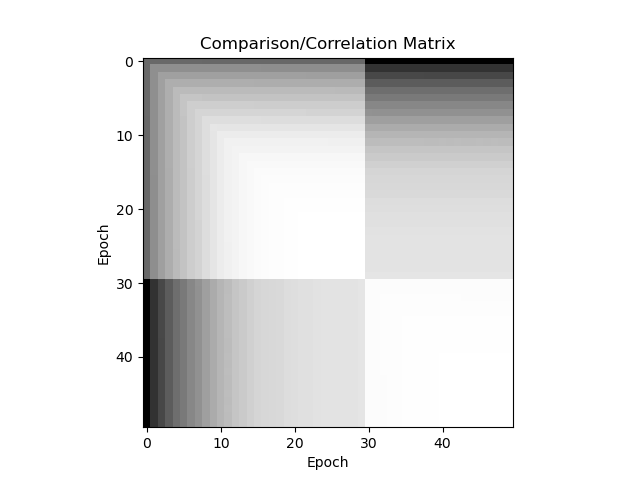
\includegraphics[width=.70\linewidth]{../Notebooks/ComparisonMatrix.png}
    \caption{Comparison Matrix for a CNN on CIFAR-10}
    \label{fig:comparison_matrix}
\end{figure}
\begin{enumerate}
    \item[\textbullet] Not fruitful! One reason is this behaves like \(\langle U,V\rangle\), where \(U,V\) are uniform on the sphere (comes from normalized Gaussians), but the variance of this is like \(1/d\), where \(d\) is dimension (very large). 
\end{enumerate} \vspace*{-1cm}
\section*{Starting Counterexample Search}\vspace{-.4cm}
\begin{figure}[H]
    \centering 
    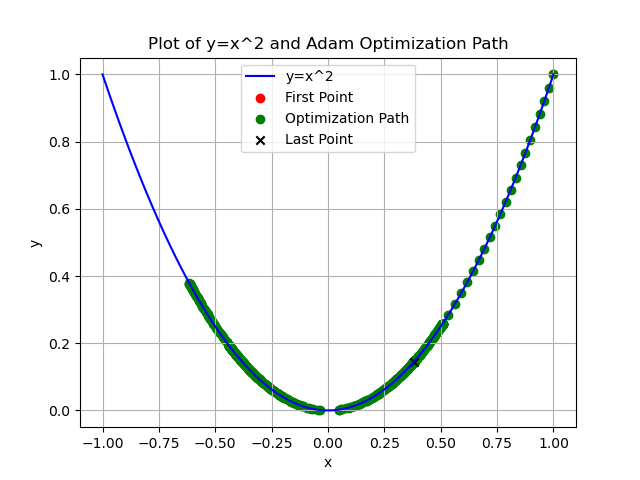
\includegraphics[width=.47\linewidth]{../Notebooks/adam_bad_initial.png}
    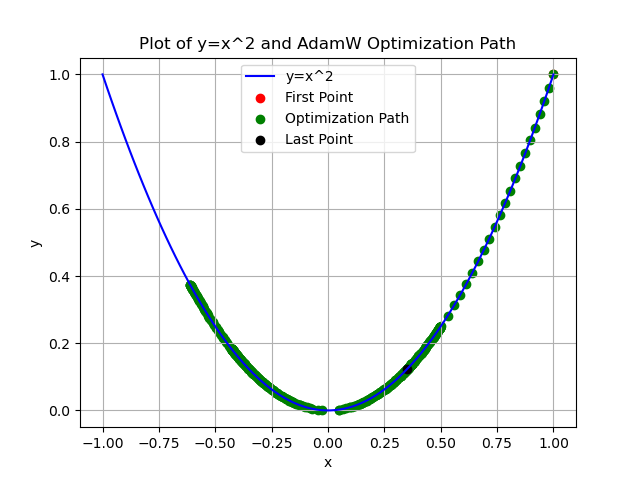
\includegraphics[width=.47\linewidth]{../Notebooks/adamw_bad_initial.png}
    \caption{\(\beta_1=.999,\beta_2 = 0.001\) leads to bad convergence}
    \label{fig:first_counterexamples}
\end{figure}
I started searching for counterexamples with simple functions and bad \(\beta_1,\beta_2\) parameters. This was easily found in figure \ref{fig:first_counterexamples}. 
Obvious, but it gives hope. In theorem 3 of \cite{reddi2019convergence}, the authors describe an avenue for Adam failing by variation in the gradients. In effect, Adam will have to memorize more than a single momentum parameter. 
My second attempt to get a counterexample was looking at quadratics of the form \(\alpha x^2 + \beta y^2\) with large deviation in \(\alpha,\beta\). These are shown below in Figure \ref{fig:optim_2d}. 
\begin{figure}[H]
    \centering 
    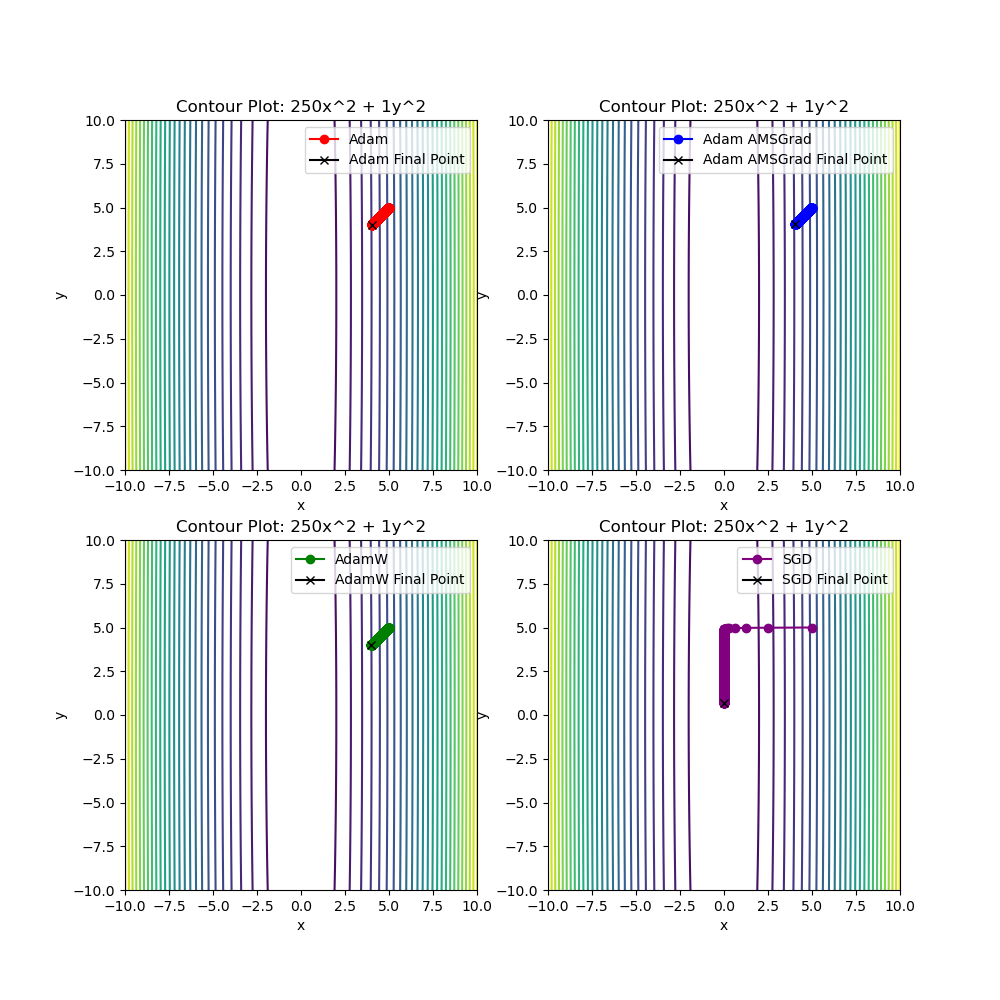
\includegraphics[width=.9\linewidth]{../Notebooks/Optimizer_behavior_2d.png}
    \caption{Optimizer Behavior with 1000 iterations and initial point (5,5)}
    \label{fig:optim_2d}
\end{figure}
Note that this was using default parameters, and the high variance slows the adaptive methods to a crawl (akin to walking slowly down a steep hill). This is because \(\Delta \theta_t \sim \nabla f(\theta_t)\) for SGD, and the changes are slower for Adam. I could not find a general convex function where Adam fails to converge, so I had to turn to online learning methods. \newpage  
\section*{Regret and Online Convex Optimization}
In online convex optimization, the learner makes a prediction \(x_t\), receives the convex loss function \(f_t(\cdot)\) and incurs a loss \(f_t(x_t)\). For some intuition think about 
\begin{align*}
\min\{f(x)\}+\min\{g(x)\}\leq \min\{f(x)+g(x)\},
\end{align*}
so if we could do a minibatch-wise optimization, it could be better than doing this after accumulation. The optimization problem is now given by the regret \(R\) of algorithm \(\calA\) in 
\begin{align*}
R_T(\calA) = \sum_{t=1}^T f_t(\theta_t) - \min_{\theta\in C} \sum_{t=1}^T f_t(\theta),
\end{align*}
where \(C\) is the convex set where our weights belong. Average regret, \(R_T/T\) compares our average distance to the optimal value, so we want \(R_T = o(T)\). In general, we know SGD can do online learning in \(\bigO(\sqrt{T})\) (\cite{langford2009slow}) for bounded subgradients. In section 3 of \cite{reddi2019convergence}, the authors show Adam can have constant average regret (not learn!) with any constant \(C>2\) and 
\begin{align*}
f_t(x) = \begin{cases}
    Cx, & t\mod 3 = 1\\ 
    -x, & \text{else}
\end{cases}\qquad \text{convex domain: }[-1,1]
\end{align*}
\section*{Theory}
The authors show \(x_t>0\) and very often \(x_t=1\), staying away from the optimal \(x=-1\). Originally, I thought AdamW would decay \(x_t\downarrow 0\) in the limit and therefore provide a better solution, but I modified the proof in \cite{reddi2019convergence} to work for AdamW (under default weight decay, although other levels may work). In fact, for some cases (like decaying step size), the proof shows that all the iterates \(x_t>1/2\) for both Adam and AdamW, meaning we can actually create a more natural sequence of functions 
\begin{align*}
g_t(x) = \1_{t\pmod{3} = 1}\begin{cases}
    Cx^2, &  0\leq x \leq 1/2  \\
    Cx ,   &1/2 < x \leq 1  \\
\end{cases} + \1_{t\pmod{3} \neq 1}\begin{cases}
    -x^2, &    0\leq x \leq 1/2 \\ 
    -x , &  1/2 < x \leq 1
\end{cases}
\end{align*}
which are quadratic until it hits \(1/2\), when they become linear. I did have to weaken the assumptions to \(3C>8\) instead of \(C>2\) from Reddi et. al., but this is minor. For the proof of the first case see the report pdf in the folder, but for the intuition think about one large gradient step (from \(C\)) followed by stepping up twice with positive gradient updates (from \(-x\)). 
\section{Numerical Verification}
I tested the prior \(f_t\) with \(C=4\) (to satisfy my stronger condition) and \(\beta_1=0,\beta_2 = 1/(1+C^2)\) which satisfies the qualifications for theorem 4.1 in \cite{kingma2017adam} for all iterations up to 10000. Each iteration I calculated the average regret and the guessed \(x_t\) value. Results are shown below in Figure \ref{fig:avg_regret}. 
\begin{figure}[H]
    \centering 
    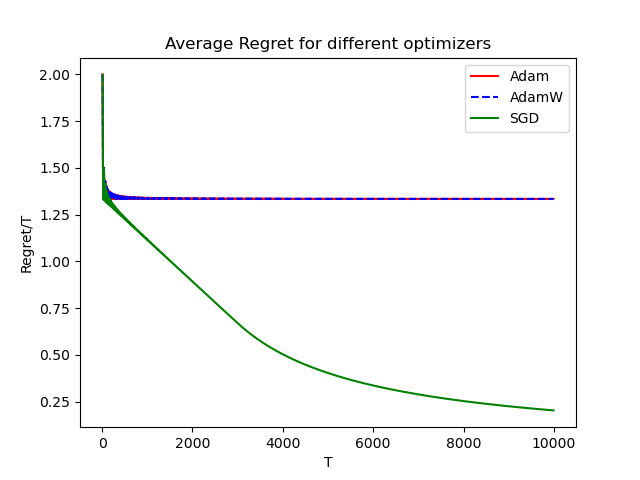
\includegraphics[width=.49\linewidth]{../Notebooks/average_regret.png}
    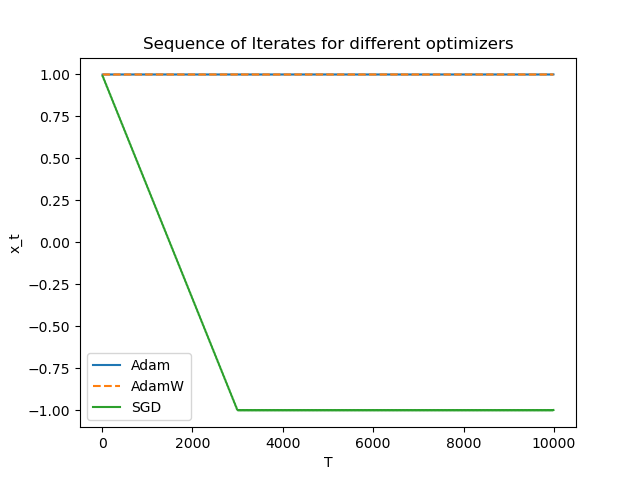
\includegraphics[width=.49\linewidth]{../Notebooks/sequence_of_iterates.png}
    \caption{Average Regret and Iterates for Different Optimizers}
    \label{fig:avg_regret}
\end{figure}
We have the expected convergence of SGD reasonably following the bound, but we see both Adam and AdamW (default weight decay) failing to learn. The iterates also clearly stay far away from the bound of \(1/2\) as predicted in the theory, with variance around \(2\times 10^{-7}\) for Adam and AdamW, but SGD does indeed converge to the optimal solution. With more weight decay AdamW does indeed start to find \(x=0\), but the threshold I found numerically was around \(20\%\) weight decay (less than my guarantee) which is not only impractical, also it only works because the optimal point is in the same direction as 0 w.r.t. \(x_t\). Since this problem is translation invariant, we could translate everything far away so AdamW could behave worse. 
\printbibliography
\end{document}